\section{真空、隧穿、瞬子与自发对称性破缺}
\subsection{量子力学中的双势阱问题}
我们先考虑量子力学中的双势阱, 看看经典的两个简并极小值在量子理论中会发生什么. 取$\hbar=m=1$, 考虑
\begin{equation}
    H=\frac{p^2}{2}+U(x),\qquad
    U(x)=\frac{\omega^2}{8a^2}(x^2-a^2)^2,\qquad a,\omega>0.
\end{equation}
这个势在$x=\pm a$处有两个极小值, 并且
\begin{equation}
    U(\pm a)=0,\qquad U''(\pm a)=\omega^2.
\end{equation}
因此在每个极小值附近, 都可以先将系统看成频率为$\omega$的简谐振子. 如果完全忽略两个势阱之间的隧穿, 就会得到两个能量均约为$\omega/2$的局域基态, 作为这个理论的低能有效近似. 接下来我们将利用路径积分计算隧穿如何使这两个能级发生劈裂, 也就是这俩近似的基态中存在隧穿.

实时间传播子为
\begin{equation}
    G(x_f,t_f;x_i,t_i)
    =\bra{x_f}\exp{-iH(t_f-t_i)}\ket{x_i}
    =\int_{x(t_i)=x_i}^{x(t_f)=x_f}\mathcal Dx\exp{iS[x]},
\end{equation}
其中
\begin{equation}
    S[x]=\int_{t_i}^{t_f}\d t\left[\frac12\left(\frac{\d x}{\d t}\right)^2-U(x)\right].
\end{equation}
作Wick旋转$t=-i\tau$, 则$iS=-S_E$, 从而得到欧氏传播子
\begin{equation}\label{ssb-euclidean-kernel}
    G_E(x_f,T;x_i,0)
    =\bra{x_f}\exp{-HT}\ket{x_i}
    =\int_{x(0)=x_i}^{x(T)=x_f}\mathcal Dx\exp{-S_E[x]},
\end{equation}
其中
\begin{equation}
    S_E[x]=\int_0^T\d\tau\left[\frac12\dot x^2+U(x)\right],
    \qquad \dot x=\frac{\d x}{\d\tau}.
\end{equation}
以下上点均表示对欧氏时间$\tau$求导. 欧氏作用量的驻点满足
\begin{equation}
    \ddot x=U'(x)=-\frac{\d[-U(x)]}{\d x}.
\end{equation}
也就是说, 寻找欧氏经典轨道等价于考虑粒子在翻转势$-U(x)$中的经典运动. 原来的两个势阱底部变成了两个山顶, 因而可以找到从一个山顶运动到另一个山顶的轨道. 这里做Wick rotation纯粹就是一个数学技巧, 方便我们从计算中提取我们需要的物理量, 而并不具有温度之类的物理含义. 在这里我们主要是想要其的两个优点: 1. Wick rotation后, 势能曲线上下翻转, 因此量子的隧穿可以变成经典的运动, 从而方便我们计算路径积分时利用鞍点近似, 将其近似为经典路径附近的Gaussian涨落. 2. 当我们计算出这俩基态间的传播子$\braket{L|\exp{-H\tau}|R}$后, 我们可以直接通过读取其中的指数$\exp{-ET}$来得到劈裂的能级.

\begin{figure}[!htbp]
    \centering
    \begin{subfigure}{0.46\textwidth}
        \centering
        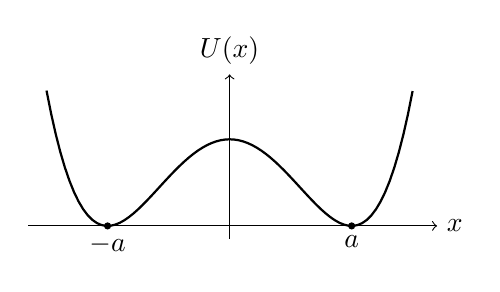
\begin{tikzpicture}[x=1.55cm,y=1.1cm]
            \draw[->] (-1.65,0) -- (1.7,0) node[right] {$x$};
            \draw[->] (0,-0.15) -- (0,1.75) node[above] {$U(x)$};
            \draw[thick,domain=-1.5:1.5,samples=81] plot (\x,{(\x*\x-1)^2});
            \fill (-1,0) circle (1.3pt) node[below] {$-a$};
            \fill (1,0) circle (1.3pt) node[below] {$a$};
        \end{tikzpicture}
        \caption{双势阱}
    \end{subfigure}\hfill
    \begin{subfigure}{0.46\textwidth}
        \centering
        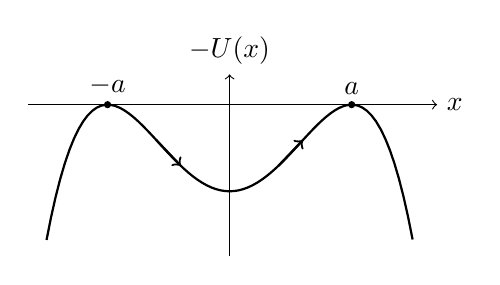
\begin{tikzpicture}[x=1.55cm,y=1.1cm]
            \draw[->] (-1.65,0) -- (1.7,0) node[right] {$x$};
            \draw[->] (0,-1.75) -- (0,0.35) node[above] {$-U(x)$};
            \draw[thick,domain=-1.5:1.5,samples=81] plot (\x,{-(\x*\x-1)^2});
            \fill (-1,0) circle (1.3pt) node[above] {$-a$};
            \fill (1,0) circle (1.3pt) node[above] {$a$};
            \draw[->,thick] (-0.6,-0.4096) -- (-0.4,-0.7056);
            \draw[->,thick] (0.4,-0.7056) -- (0.6,-0.4096);
        \end{tikzpicture}
        \caption{欧氏经典运动对应的翻转势}
    \end{subfigure}
    \caption{双势阱及其翻转势. 欧氏轨道连接翻转势的两个山顶.}
    \label{fig:ssb-double-well}
\end{figure}

先在整条欧氏时间轴上寻找有限作用量的轨道, 要求
\begin{equation}
    x(-\infty)=-a,\qquad x(+\infty)=a,\qquad
    \dot x(\pm\infty)=0.
\end{equation}
欧氏运动方程有守恒量
\begin{equation}
    \frac12\dot x^2-U(x)=0,
\end{equation}
于是解得
\begin{equation}\label{ssb-instanton-solution}
    x_0(\tau)=a\tanh\left[\frac\omega2(\tau-\tau_0)\right].
\end{equation}
这就是瞬子(Instanton), $\tau_0$是瞬子中心. 它主要在宽度约为$\omega^{-1}$的欧氏时间区间内完成跃迁; 反向的轨道$-x_0(\tau)$则是反瞬子(Anti-instanton).

利用$\dot x_0^2=2U(x_0)$, 单瞬子的作用量为
\begin{align}\label{ssb-instanton-action}
    S_0\equiv S_E[x_0]
    &=\int_{-\infty}^{+\infty}\d\tau\,\dot x_0^2
      =\int_{-a}^{a}\d x\sqrt{2U(x)}\notag\\
    &=\frac\omega{2a}\int_{-a}^{a}\d x\,(a^2-x^2)
      =\frac23\omega a^2.
\end{align}
因此一次瞬子事件会带来指数压低因子$\exp{-S_0}$. 以下考虑$S_0\gg1$的半经典区域, 并在$\omega T\gg1$的长时间区间中使用这个解.

\note[瞬子解中的无穷时间]{
式\eqref{ssb-instanton-solution}严格地说满足的是$\tau\to\pm\infty$的边界条件, 它不会在有限时间恰好到达$x=\pm a$. 在很长的有限区间$[0,T]$内, 当瞬子中心远离两端时, 可以用它近似描述一次跃迁, 忽略端点附近的修正. 后面出现的$\int\d\tau_0\simeq T$正是在这个意义下成立的.
}

只有$\exp{-S_0}$还不够, 我们还需要计算瞬子附近的涨落. 写成
\begin{equation}
    x(\tau)=x_0(\tau)+\delta x(\tau),
\end{equation}
对作用量作泛函Taylor展开:
\begin{align}
    S_E[x_0+\delta x]
    &=S_0+\int\d\tau\,
      \left.\frac{\delta S_E}{\delta x(\tau)}\right|_{x_0}\delta x(\tau)\notag\\
    &\quad+\frac12\int\d\tau_1\d\tau_2\,
      \left.\frac{\delta^2S_E}{\delta x(\tau_1)\delta x(\tau_2)}\right|_{x_0}
      \delta x(\tau_1)\delta x(\tau_2)+\cdots.
\end{align}
一阶项由于$x_0$满足经典运动方程而消失. 对固定端点的变分, 有
\begin{align}
    \frac{\delta S_E}{\delta x(\tau)}
    &=U'(x(\tau))-\ddot x(\tau),\\
    \left.\frac{\delta^2S_E}{\delta x(\tau_1)\delta x(\tau_2)}\right|_{x_0}
    &=\left[U''(x_0(\tau_1))-\frac{\d^2}{\d\tau_1^2}\right]
      \delta(\tau_1-\tau_2).
\end{align}
于是二阶项可以写成
\begin{equation}\label{ssb-quadratic-fluctuation}
    S_E[x_0+\delta x]
    =S_0+\frac12\int\d\tau\,\delta x\mathcal M_\tau\delta x+\cdots,
\end{equation}
其中涨落算符为
\begin{align}\label{ssb-fluctuation-operator}
    \mathcal M_\tau
    &=-\frac{\d^2}{\d\tau^2}+U''(x_0(\tau))\notag\\
    &=-\frac{\d^2}{\d\tau^2}+\frac{\omega^2}{2a^2}(3x_0^2-a^2)\notag\\
    &=-\frac{\d^2}{\d\tau^2}+\omega^2
      -\frac{3\omega^2}{2\cosh^2[\omega(\tau-\tau_0)/2]}.
\end{align}
% 手稿待核查：第一页末保留了二阶项的 1/2，第二页首行的 Gaussian 指数未写 1/2。
% 此处保留第一页的 Taylor 展开；两页原式的不一致另见 errors.md。
若将涨落展开到正交归一的本征函数上,
\begin{equation}
    \mathcal M_\tau\psi_n=\lambda_n\psi_n,\qquad
    \int\d\tau\,\psi_n\psi_m=\delta_{nm},\qquad
    \delta x=\sum_n c_n\psi_n,
\end{equation}
则二阶项变成$\frac12\sum_n\lambda_nc_n^2$. 对每个非零的正本征值, Gaussian积分给出
\begin{equation}
    \int\frac{\d c_n}{\sqrt{2\pi}}\exp{-\frac12\lambda_nc_n^2}
    =\lambda_n^{-1/2}.
\end{equation}
因此非零模的贡献正比于$\prod_{n\ne0}\lambda_n^{-1/2}=(\det'\mathcal M_\tau)^{-1/2}$, 撇号表示去掉零本征值. 路径积分测度的共同归一化将在与简谐振子的比较中确定.

这里不能直接把所有模都当作普通的Gaussian积分, 因为移动瞬子中心$\tau_0$并不改变它在无穷时间轴上的作用量. 对运动方程再求一次导数, 就得到
\begin{equation}
    \mathcal M_\tau\dot x_0
    =-\dddot x_0+U''(x_0)\dot x_0=0.
\end{equation}
所以$\dot x_0$是零模. 根据式\eqref{ssb-instanton-action}, 可以将归一化的零模取为
\begin{equation}
    \psi_0(\tau)=-\frac{\dot x_0(\tau)}{\sqrt{S_0}},\qquad
    \int\d\tau\,\psi_0^2=1.
\end{equation}
另一方面, 瞬子中心移动$\d\tau_0$所引起的变化为
\begin{equation}
    \delta x_0=\frac{\partial x_0}{\partial\tau_0}\d\tau_0
    =-\dot x_0\d\tau_0=\psi_0\d c_0.
\end{equation}
于是$\d c_0=\sqrt{S_0}\d\tau_0$, 原本的零模积分应改成对瞬子中心的积分:
\begin{equation}\label{ssb-zero-mode-measure}
    \int\frac{\d c_0}{\sqrt{2\pi}}
    =\sqrt{\frac{S_0}{2\pi}}\int\d\tau_0
    \simeq\sqrt{\frac{S_0}{2\pi}}\,T.
\end{equation}
这就是单瞬子贡献中$T$的来源: 瞬子可以发生在整个时间区间中的任意位置. 有限区间的端点会破坏严格的平移零模, 这里按长时间极限处理它.

为了确定其余的归一化, 与同一时间区间上、具有相同固定端点涨落边界条件的简谐振子作比较. 势阱底部的参考算符为
\begin{equation}
    \mathcal M_0=-\frac{\d^2}{\d\tau^2}+\omega^2.
\end{equation}
在Gaussian近似下, 没有瞬子的传播因子就是以势阱底部为原点的简谐振子传播核:
\begin{equation}\label{ssb-no-instanton-kernel}
    K_0(T)=\left(\frac{\omega}{2\pi\sinh\omega T}\right)^{1/2}
    \underset{\omega T\gg1}{\simeq}\sqrt{\frac\omega\pi}\exp{-\omega T/2}.
\end{equation}
这里$K_0$中的下标表示零次瞬子事件. 将它提出后, 瞬子对非零模涨落的改变由行列式之比描述. 两个行列式采用同一正则化, 去掉瞬子的平移模后再取长时间极限. 对当前四次势, 其结果为
\begin{equation}\label{ssb-determinant-ratio}
    \frac{\det'\mathcal M_\tau}{\det\mathcal M_0}
    =\frac{1}{12\omega^2}.
\end{equation}
% 手稿待核查：原稿将 1/sqrt(det' M_tau) 直接写成 sqrt(12) omega，
% 未显式注明相对简谐振子的归一化；此处单列参考算符，待本人确认，见 errors.md。
将零模与非零模的贡献合在一起, 定义
\begin{equation}\label{ssb-instanton-prefactor}
    k=\sqrt{\frac{S_0}{2\pi}}
      \left(\frac{\det\mathcal M_0}{\det'\mathcal M_\tau}\right)^{1/2}
      =\omega\sqrt{\frac{6S_0}{\pi}}.
\end{equation}
于是单瞬子给出的异阱传播贡献为
\begin{equation}\label{ssb-one-instanton-kernel}
    G_E(a,T;-a,0)\big|_{\text{单瞬子}}
    \simeq K_0(T)\,kT\exp{-S_0}.
\end{equation}
取行列式之比的意义, 就是将整段时间内已有的简谐振子涨落提取到$K_0(T)$中, 只计算插入一次瞬子后增加的权重$k\exp{-S_0}\d\tau_0$. 这里的$k$是前因子, 尚未包含指数压低因子$\exp{-S_0}$.

路径积分包含任意次来回跃迁. 当相邻瞬子或反瞬子的间距远大于$\omega^{-1}$时, 可以忽略它们之间的相互作用, 将总作用量近似写成各次事件作用量之和. 这就是稀薄瞬子气体近似(Dilute Instanton Gas Approximation).

从左阱出发, 瞬子与反瞬子必须交替出现:
\begin{equation}
    -a\xrightarrow{I}a\xrightarrow{\bar I}-a\xrightarrow{I}a\cdots.
\end{equation}
% 手稿待核查：原稿先写 n 个 instanton 和 n-1 个 anti-instanton，
% 下一行却写 (k T exp(-S_E))^n/n!；事件总数与该处 n 的含义不一致。
% 原稿这一中间式保留在此，未作为已核实等式排入正文；见 errors.md。
以下用$N$表示瞬子与反瞬子的\emph{总数}. 对于给定的时间顺序
\begin{equation}
    0<\tau_1<\tau_2<\cdots<\tau_N<T,
\end{equation}
对所有中心位置积分给出
\begin{equation}
    \int_0^T\d\tau_N\int_0^{\tau_N}\d\tau_{N-1}\cdots
    \int_0^{\tau_2}\d\tau_1=\frac{T^N}{N!}.
\end{equation}
这里将稀薄配置的积分区域近似延伸到了整个有序区域, 忽略瞬子重叠的修正. 因而$N$次事件的贡献为
\begin{equation}\label{ssb-many-instanton-kernel}
    K_N(T)\simeq K_0(T)\frac{\big(kT\exp{-S_0}\big)^N}{N!}.
\end{equation}
这里的$K_0$表示在到达某个近似真空态后在最低点附近的震荡, 由于我们认为$T\gg\omega^{-1}$, 因此瞬子的传播时间可以忽略不计, 将所有的基态处的振荡都算上, 总共就是振荡了$T$的时间, 因此总共贡献一个$K_0(T)$.

同阱传播要求$N$为偶数, 异阱传播要求$N$为奇数, 所以求和得到
\begin{align}\label{ssb-instanton-sum}
    G_E(-a,T;-a,0)
    &\simeq K_0(T)\sum_{n=0}^\infty
      \frac{\big(kT\exp{-S_0}\big)^{2n}}{(2n)!}\notag\\
    &=K_0(T)\cosh\big(kT\exp{-S_0}\big),\notag\\
    G_E(a,T;-a,0)
    &\simeq K_0(T)\sum_{n=0}^\infty
      \frac{\big(kT\exp{-S_0}\big)^{2n+1}}{(2n+1)!}\notag\\
    &=K_0(T)\sinh\big(kT\exp{-S_0}\big).
\end{align}
然后将异阱传播子的双曲正弦展开, 得到
\begin{align}
    G_E(a,T;-a,0)
    &\simeq\sqrt{\frac\omega\pi}\exp{-\omega T/2}
      \sinh\big(kT\exp{-S_0}\big)\notag\\
    &=\frac12\sqrt{\frac\omega\pi}
      \left[\exp{-\left(\frac\omega2-k\exp{-S_0}\right)T}
      -\exp{-\left(\frac\omega2+k\exp{-S_0}\right)T}\right].
\end{align}
另一方面, 插入能量本征态, 欧氏传播子具有谱展开
\begin{equation}
    G_E(a,T;-a,0)
    =\sum_n\braket{a|n}\braket{n|-a}\exp{-E_nT}.
\end{equation}
比较指数中的能量, 就可以读出在当前近似下最低的两个能级:
\begin{equation}\label{ssb-double-well-energies}
    E_0\simeq\frac\omega2-k\exp{-S_0},\qquad
    E_1\simeq\frac\omega2+k\exp{-S_0}.
\end{equation}
因此
\begin{important}
    \begin{align}
        \Delta E\equiv E_1-E_0
        &\simeq2k\exp{-S_0}
        =2\omega\sqrt{\frac{6S_0}{\pi}}\exp{-S_0},\notag\\
        S_0&=\frac23\omega a^2.
    \end{align}
\end{important}
式\eqref{ssb-double-well-energies}中的共同能量$\omega/2$只是单阱的简谐近似; 非谐项还会给两个能级带来相同的微扰修正. 瞬子计算所揭示的是它们之间指数小的能级劈裂, 而非两个绝对能量的全部修正.

若用$\ket L,\ket R$表示低能近似下分别局域在左右势阱中的归一化态, 则最低的两个能量本征态近似为
\begin{equation}
    \ket0\simeq\frac{\ket L+\ket R}{\sqrt2},\qquad
    \ket1\simeq\frac{\ket L-\ket R}{\sqrt2}.
\end{equation}
这里的局域态是波包, 与前面用于定义传播核的位置本征态$\ket{x=\pm a}$不同. 基态是偶宇称态, 第一激发态是奇宇称态. 因而对于有限参数下的这个双势阱, 两个经典极小值并不意味着两个简并的量子基态; 隧穿使它们混合, 形成一个非简并的对称基态.

\note[欧氏瞬子为何对应实时间隧穿]{
欧氏传播子与实时间传播子包含同一组能量和本征态, 只是谱展开中的$\exp{-E_nT}$变为$\exp{-iE_nt}$. 在上述两态近似中, 从$\ket L$出发得到
\begin{equation}
    \bra R\exp{-iHt}\ket L
    \simeq i\exp{-i\bar E t}\sin\left(\frac{\Delta E}{2}t\right),
    \qquad \bar E=\frac{E_0+E_1}{2},
\end{equation}
因此$P_{L\to R}(t)\simeq\sin^2(\Delta E\,t/2)$. 这说明欧氏瞬子计算得到的能级劈裂, 在实时间中正对应左右势阱之间的量子隧穿. 作解析延拓的是传播振幅的时间依赖; 无需将单条欧氏瞬子轨道解释成实时间中的实经典轨道.
}

\subsection{实标量场中的双势阱}
现在将上一节的双势阱推广到实标量场. 先把系统放在体积为$V$的连通空间区域$\Omega$内, 并采用周期边界条件, 使两个均匀的场构型都被允许. 考虑
\begin{equation}
    \mathcal L=\frac12\partial_\mu\phi\partial^\mu\phi-U(\phi),
    \qquad U(\phi)=\frac{\omega^2}{8a^2}(\phi^2-a^2)^2,
    \qquad a,\omega>0.
\end{equation}
这里沿用上一节势函数的形式, 但$a$现在具有场的量纲, $U$是势能密度, 而$\omega^2=U''(\pm a)$是经典真空附近小涨落的质量平方. 理论具有$\mathbb Z_2$对称性$\phi\to-\phi$, 两个经典真空是整个空间上均匀的$\phi=\pm a$. 我们仍在半经典近似适用的区域内讨论它们之间的隧穿.

Wick旋转后, 场的欧氏作用量为
\begin{equation}\label{ssb-field-euclidean-action}
    S_E^{\mathrm{field}}[\phi]
    =\int_{-\infty}^{+\infty}\d\tau\int_\Omega\d^3x
      \left[\frac12(\partial_\tau\phi)^2
      +\frac12(\nabla\phi)^2+U(\phi)\right].
\end{equation}
要计算两个均匀真空之间的跃迁, 应对每个空间点施加
\begin{equation}\label{ssb-field-instanton-boundary}
    \phi(\mathbf x,-\infty)=-a,\qquad
    \phi(\mathbf x,+\infty)=a.
\end{equation}
我们要找的是满足这组边界条件的所有场构型中, 欧氏作用量最小的那个. 不能仅凭空间梯度项非负就直接假设$\phi$与空间无关, 因为还需要证明其余两项也能同时达到下界.

为此, 定义
\begin{equation}
    \begin{gathered}
        F(\phi)=\frac\omega{2a}(a^2-\phi^2),\qquad
        W(\phi)=\frac\omega{2a}\left(a^2\phi-\frac{\phi^3}{3}\right),\\
        W'(\phi)=F(\phi),\qquad U(\phi)=\frac12F(\phi)^2.
    \end{gathered}
\end{equation}
将欧氏时间动能与势能配方, 得到
\begin{align}\label{ssb-field-action-bound}
    S_E^{\mathrm{field}}[\phi]
    &=\frac12\int\d\tau\int_\Omega\d^3x
      \left[(\partial_\tau\phi-F(\phi))^2+(\nabla\phi)^2\right]
      +\int_\Omega\d^3x\int\d\tau\,\partial_\tau W(\phi)\notag\\
    &=\frac12\int\d\tau\int_\Omega\d^3x
      \left[(\partial_\tau\phi-F(\phi))^2+(\nabla\phi)^2\right]
      +V\big[W(a)-W(-a)\big]\notag\\
    &\geq V\frac23\omega a^2.
\end{align}
最后一项只取决于时间两端的边界值, 因此这个下界对中间任意非均匀的场构型都成立. 等号成立当且仅当
\begin{equation}
    \nabla\phi=0,\qquad \partial_\tau\phi=F(\phi).
\end{equation}
第一条说明整个连通空间中的场必须一起变化, 即$\phi(\mathbf x,\tau)=\phi(\tau)$; 第二条恰好就是上一节的瞬子方程, 所以
\begin{equation}\label{ssb-field-instanton}
    \phi_0(\mathbf x,\tau)
    =a\tanh\left[\frac\omega2(\tau-\tau_0)\right].
\end{equation}
所有空间点具有同一个瞬子中心$\tau_0$. 若让不同位置先后跃迁, 就会引入空间梯度, 无法达到上述下界. 因此这个均匀瞬子确实是在给定跃迁边界条件下的全局极小值, 而不只是一个猜出来的驻点.

这里的稳定性也可以直接从配方后的作用量看出. 令$\phi=\phi_0+\eta$, 其中$\eta$在时间两端消失, 则二阶展开为
\begin{equation}
    \begin{aligned}
        &S_E^{\mathrm{field}}[\phi_0+\eta]
        -S_E^{\mathrm{field}}[\phi_0]\\
        &\qquad=\frac12\int\d\tau\int_\Omega\d^3x
          \left[(\partial_\tau\eta-F'(\phi_0)\eta)^2
          +(\nabla\eta)^2\right]+O(\eta^3).
    \end{aligned}
\end{equation}
二次型非负, 因而没有负模; 整体平移$\tau_0$仍给出一个零模. 这里所说的稳定是欧氏作用量在固定跃迁边界条件下的稳定性.

既然最小作用量构型与空间无关, 将它代回式\eqref{ssb-field-euclidean-action}, 空间积分便只贡献体积因子:
\begin{align}\label{ssb-field-volume-factor}
    S_E^{\mathrm{field}}[\phi(\tau)]
    &=V\int_{-\infty}^{+\infty}\d\tau
      \left[\frac12\dot\phi^2+U(\phi)\right]
      \equiv V S_E[\phi],\notag\\
    S_E^{\mathrm{field}}[\phi_0]
    &=V S_0,\qquad S_0\equiv S_E[\phi_0]=\frac23\omega a^2.
\end{align}
这里的$S_E$就是上一节量子力学欧氏作用量的同形式泛函, 只需将$x(\tau)$换成$\phi(\tau)$. 注意在当前场论量纲下, $S_0$是单位空间体积的瞬子作用量, 无量纲的隧穿指数是$VS_0$. 这一步只约化了均匀构型的作用量, 完整场论的路径积分仍包含非均匀涨落.

于是一次从$\phi=-a$到$\phi=+a$的整体隧穿, 在主导半经典指数上受到
\begin{equation}
    \exp{-S_E^{\mathrm{field}}[\phi_0]}=\exp{-VS_0}
\end{equation}
的压低. 与上一节相同, 在稀薄瞬子气体近似下, 有限体积中两个近似真空的混合使最低两个能级发生劈裂:
\begin{equation}\label{ssb-field-energy-splitting}
    \Delta E(V)\simeq2k_V\exp{-VS_0}.
\end{equation}
这里$k_V$表示场论涨落给出的因子, 不能直接照搬量子力学中的$k$, 因为还存在所有非零空间动量的涨落模. 上式展示的是经典瞬子给出的主导指数; 量子修正可以修正指数中单位体积作用量的系数. 在我们讨论的半经典破缺相中, 这一系数保持为正, 隧穿劈裂随体积增大而指数趋零.

有限$V$时, 两个近似真空仍会混合, 真正的基态仍是$\mathbb Z_2$对称的组合. 但在无限体积极限下,
\begin{equation}
    V\to\infty:\qquad
    S_E^{\mathrm{field}}[\phi_0]\to\infty,\qquad
    \Delta E(V)\to0.
\end{equation}
此时整个空间从一个真空翻转到另一个真空的隧穿被压低到零, 隧穿时间尺度$1/\Delta E$发散. 分别局域在两个势阱附近的态便对应两个简并的真空, 其场的期望值在主导半经典近似下为$\langle\phi\rangle\simeq\pm a$, 并由$\mathbb Z_2$变换相互交换. 选择其中一个真空, 就自发破坏了这个对称性.

\begin{important}
    对这里的实标量场双势阱, 有限体积中的隧穿会解除两个近似真空的简并, 而无限体积极限使隧穿消失, 允许两个真空严格简并. 因此, 自发对称性破缺所对应的这种简并基态, 是无限体积量子场论的特性.
\end{important}
